\section{SEAC mission and project relevance}
Unilever's Safety and Environmental Assurance Centre (SEAC) division was founded in 1990 for assessing the safety and environmental impact of Unilever products. SEAC scientists work together with government scientists, regulators, and academics to carry out pioneering approaches that span different scientific fields -- \textit{i.e.} toxicology, microbiology, computational chemistry, bioinformatics, and mathematical modelling -- in order to ensure that Unilever products are safe for use and consumption as well as for the environment \citep{unileverLeadingSafetyEnvironmental2023}.

Unilever has a long history of promoting the use of non-animal testing methods for risk assessment, while trying to develop sustainable and viable alternatives, such as \textit{in vitro} assays and computational modelling \citep{unileverAlternativesAnimalTesting2023}. Besides the ethical discussion of which I will not enter into the merits, there is also scientific evidence to support the need for non-animal testing: many review studies reported that results from tests conducted in mouse, rat, and rabbit models are highly inconsistent in predicting toxic responses in humans \citep{vannormanLimitationsAnimalStudies2020}. Historically, there have been cases of drugs that were previously deemed safe during the clinical trial phases, and later had to be recalled for causing adverse effects, such as Vioxx from Merck which increases the risk of cardiovascular morbidity and mortality, and caused 38000 deaths and 88000 induced heart attacks \citep{juniRiskCardiovascularEvents2004}. Other notable cases include Thalidomide, which was withdrawn because it causes phocomelia and fetal deformations in pregnant women, despite there being no teratogenic effect reported in animal models, and Isuprel, which was originally developed for the treatment of asthma and caused an increase in deaths due to the high dosage approved in countries like the United Kingdom, Ireland, Australia and New Zealand \citep{jalbaThreeGenerationsOngoing2008}. Conversely, the opposite is also true: there are examples of safe drugs which are readily available that would have never passed toxicity testing if conducted in animal models, such as aspirin (that causes reproductive abnormalities and liver toxicity in rats), and paracetamol (that is toxic for cats and dogs) \citep{vannormanLimitationsAnimalStudies2020,villarIbuprofenAspirinAcetaminophen1998}.

Another reason in support of non-animal testing is the throughput: Unilever has a portfolio of more than \num{400} brands -- comprising food products, supplements, beauty and personal care products, beverages, and home care products -- therefore using animal models for testing all the compounds in all the formulations of all their products is simply not a viable option, both in terms of economical sustainability and in time and resource spending.
% need data
Animal testing is a very low throughput assay, and relatively expensive when compared to other \textit{in vitro} assays, which, by their nature, can more easily be automated, standardized, and scaled to ideally match the required characteristics for toxicity and risk assessment. An example is the \emph{Tox21} program, a consortium of public agencies, among whose main objectives are to develop better models for predicting the toxicity of an array of substances (the current goal is set to \num{10000}), and developing new \textit{in vitro} assays to reduce, refine, and replace the use of animal models \citep{lynchHighThroughputScreeningAdvance2023}. Among these technologies, in the current phase of the Tox21 program, the focus is on mid- to high-throughput gene expression screenings using human tissues and cells.

High Throughput Transcriptomics (HTTr) is a particular RNA sequencing (RNA-seq) technique designed to evaluate gene expression changes as effects of multiple conditions, such as treatment with different chemicals, increasing concentrations, or at different time points. In fact, time is an important factor that has often been overlooked in the past, but recent developments in transcriptome studies have allowed the design of more complicated experiments -- such as longitudinal studies -- in order to capture the biological processes in whole. For example, repeated exposure to small doses of a chemical compound (chronic dosage), or a spike dosage (acute phase) followed by a ``recovering'' phase. This is where this project begins: our main goal is to leverage the power of HTTr assays for toxicity and safety assessment by developing a new pipeline for the analysis of longitudinal data.

\section{Modelling longitudinal data}
RNA-seq can be used to evaluate transcriptional changes in genes already known (present in previous databases), but also to reconstruct the full RNA transcripts, even if they were not previously annotated. The sequencing process generates millions or billions of short sequences called \emph{reads} which are smaller portions of the original transcripts. The reads must then be matched to their original position inside the genome by aligning them to a reference. From this alignment, a final count is produced for each specific region of the genome, and a \emph{count matrix} is produced containing the number of reads per gene (or ``genome portion'') per different condition included in the experiment, which correspond to how much each gene is expressed \citep{frazeeDifferentialExpressionAnalysis2014,nagalakshmiTranscriptionalLandscapeYeast2008}. This is the starting point of many analytical pipelines.

For the scope of this project, the central principle is how time can be modelled and simultaneously account for expression variation over time. The ``common'' approach consists of the determination of differentially expressed genes (DEG) among different conditions. One of the most used tools is DESeq \citep{andersDifferentialExpressionAnalysis2010} and its later implementation DESeq2 \citep{loveModeratedEstimationFold2014a}, whose assumption is that each feature is independent, including time points, therefore time is modelled as a categorical variable. The software then performs linear regression for each feature (covariate) across all genes, and a fold change is calculated, indicating how much the expression level of a gene differs compared to the null model, which is when the expression level stays the same.

One obvious issue of this approach is that time cannot always be represented as a categorical variable, and by considering it as such one may oversimplify the biological system. This is an easy implementation of the already consolidated means for analysing genomic data that do not require existing models to be readapted or changed. This interpretation may work when we have less time points or when they are very distant, for example if we are studying a well-known biological mechanism for which we expect a certain outcome only after a certain amount of time has passed, but it poorly applies to an experiment where there are several repeated measurements of the same feature, and therefore each individual measure is no longer truly independent. 

To solve this issue, a possible different approach consists in treating time as a continuous variable, and modelling the gene expression using parametric statistics. One of the tools that uses this assumption is ImpulseDE2 \citep{fischerImpulseModelbasedDifferential2018}, which uses ``pulse functions'' to model gene expression levels over time by representing the transition between an initial state to a peak state, to a steady state. The goodness of fit is then evaluated by calculating a log-likelihood ratio test. One of the limitations of this approach is the limited number of the possible functions taken into account, which could recapitulate time-dependant gene expression. A more generalized method would be finding the function with the highest likelihood given the expression data, without specifying any function. This can be achieved by using Gaussian Processes (GPs), which are a type of non-parametric non-linear regression. Example tools that apply this concept are PairGP \citep{vantiniPairGPGaussianProcess2022} and GPrank \citep{topaGPrankPackageDetecting2018}.

\section{Choice of tool}
The choice of the tool examined in this study was based on review papers in the Literature -- two in particular -- detailing methods for RNA-seq data analysis. The first is a comparative study by \citet{spiesComparativeAnalysisDifferential2019}, in which the authors compare tools developed specifically for differential expression analysis of time course data, both on simulated and biological data.
The second is a review paper by \citet{ohTemporalDynamicMethods2021}, in which the authors describe a more comprehensive list of tools and dynamic strategies for studying non-periodical and periodical time course data, \textit{de facto} enriching the list of tools from \citeauthor{spiesComparativeAnalysisDifferential2019}.

From these two papers, a list of tools and their relative original papers was compiled, which was then used in a Python script to cross-search NCBI databases for resources linked to each article. Datasets linked to each publication entry were considered for two main reasons: the importance of reproducibility and the ability to test the consistency of those tools, therefore it is crucial that the authors made their data available, and having as many datasets available as possible for benchmarking the full RNA-seq analysis pipeline of this project. Lastly, the number of citation for each tool was captured in order to develop a ranking system (for a detailed description see section \ref{papers_metric}). The result is an updated table of which table \ref{tab:oh_metric} shows the most relevant columns.

This approach has three principal shortcomings:
\begin{enumerate}
    \item To perform cross-searches among NCBI databases, the NCBI E-Utilities software needs to be provided with the relative database ID (\textit{i.e.} PMID to search the Pubmed database). The list compiled from the review papers has DOI strings, which are extra fields in a Pubmed entry and can return unexpected results, like for the case of \emph{PairGP} (last row in table \ref{tab:oh_metric}): the Pubmed search returned 0 papers cited the PairGP paper, which could not be the case since it got cited at least once by \citeauthor{ohTemporalDynamicMethods2021}. This issue is due to a double DOI corresponding to the same article: one also present in the NCBI records, and one relative to the biorXiv pre-print, which is not accessible by simply using NCBI E-utilities.
    \item The average number of citations per year was used to rank the tools, which is not an objective metric for assessing the goodness of a paper, but it gives a rough estimate of the popularity it has among the scientific community. Generally speaking, a more popular tool would get included more often in analytical pipelines than a less popular one, which in turn would result in a more solid consensus. In fact, one of the challenges the computational community is facing is that there is still no consensus for the analysis of longitudinal RNA-seq data, which is also the reason why there is such a large number of tools available.
    \item Cross-searches among NCBI databases rely on the authors (or the publishers) to correctly list the resources linked to their publication. In this case, very few Pubmed entries also had the GEO Datasets accession linked, despite having it explicitly written in the text or in the supplementary material. Another possible reason for a GEO Datasets entry to not have an article linked to it could be if the data had been submitted well in advance of the publication, and it had not been updated.
\end{enumerate}

In spite of these problems, the script returned a reasonable outcome. It is worth noting that the tools for the analysis of periodical time courses are among the most popular. It may be because circadian rhythmic and cell-cycling changes have historically been more studied, or because some of these tools have been repurposed from older applications to also adapt to this type of analysis. Either way, since the HTTr assays used in this project involve non-periodical time course data, those tools are not taken into consideration. Within the non-periodical time course tools, the tools previously suggested by Unilever's external collaborators -- maSigpro and ImpulseDE2 -- are ranked among the highest positions. Lastly, some tools actually have publicly available datasets linked to their papers.

\section{DPGP}
This study focuses on the \emph{DPGP} (\emph{Dirichlet Process Gaussian Process}) tool based on the evaluation of the results of the NCBI cross-search from the previous section and shown in table \ref{tab:oh_metric}. Among the tools for the analysis of non-periodical time course, DPGP is one of the highest ranking, but unlike the others that were design to perform differential expression analysis, it has been developed for clustering time series of transcriptional data.

Clustering can be particularly useful in analysing RNA-seq data because it can be used to visualize the results, identify potential bias in the data (such as batch effects), but also to reduce the complexity by grouping genes into sub-categories of ``expression behaviours''. Furthermore, genes that belong to a cluster can be annotated ``by association'' assuming that they must share a common feature in order to be put in the same category, \textit{e.g.} regulatory pathway, molecular function, cellular location, sequence motif, etc. \citep{walkerPredictionGeneFunction1999}.

Unlike other clustering algorithms, DPGP does not need to pre-determine the number of clusters -- like in k-means clustering -- but it uses a \emph{Dirichlet process} (DP) to infer it from the data itself, combined with a Gaussian process (GP) for modelling expression levels over time.

\subsection{Bayesian inference}
DPGP uses both Dirichlet and Gaussian processes as priors, or in other words, the initial information about the data. Priors are used in Bayesian inference to infer the posterior distribution, which can be described as the updated initial information after factoring new observation (new knowledge) from the data.

In Bayesian inference, the posterior probability is calculated with Bayes' theorem, which uses the estimate of the probability of the hypothesis before factoring the data -- prior --, and the probability of observing the data given the parameters (or the model) -- likelihood -- to get the probability of observing the parameters given the data -- posterior.

Bayes' theorem general formula is:
\begin{displaymath}
    P(H|D) = \frac{P(D|H) \cdot P(H)}{P(D)}
\end{displaymath}
where
\begin{itemize}
    \item $H$ is the ``hypothesis'' event
    \item $D$ is the ``data'' or ``information'' event
    \item $P(H|D)$ is the posterior conditional probability (probability of observing the hypothesis given the data)
    \item $P(D|H)$ is the \emph{likelihood}, or prior conditional probability (probability of observing the data given the hypothesis)
    \item $P(H)$ is the prior, and
    \item $P(D)$ is the \emph{marginal likelihood}, or the probability of the observed data.
\end{itemize}

Lastly, to estimate the posterior distribution of the parameters of the mixed DPGP model, the software uses a Markov chain Monte Carlo method -- in particular, a Gibbs sampling algorithm -- to simultaneously infer the number of clusters \emph{and} the parameters that describe the gene expression trajectories for each cluster.

\subsection{Dirichlet process}
Dirichlet processes are often used in Bayesian models as a non-parametric prior because they allow not having to determine a certain parameter -- like in this case, the number of clusters -- but lets the data itself inform that decision.

The DP can be considered as a distribution over distributions, where the latter can be parametrized as the ``mean'' of the DP, with a ``concentration'' parameter that determines how closely the sampled distributions are to the base ``mean'' distribution.

DP can be used for clustering because distributions sampled from a DP can be considered an isolated group (or cluster) from which the data comes from.

\begin{figure}[!ht]
    \centering
    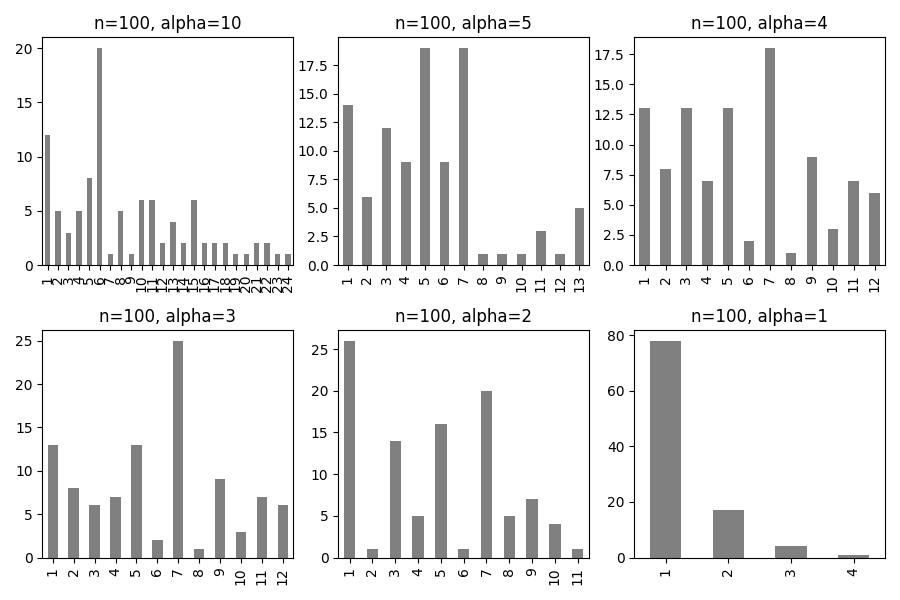
\includegraphics[width=.9\textwidth]{src/chinese_restaurant.png}
    \caption[Chinese restaurant process example]{Chinese restaurant process example. The picture shows the effect of the concentration parameter $\alpha$, which affects the probability of creating a new group -- or table, or cluster -- with a fix number to be organized. Each bar represents the number of assigned values to that group. As the $\alpha$ value decreases, also the number of groups gets lower, with a maximum of 24 groups for $\alpha=10$, and a minimum of 4 for $\alpha=1$. The default value used in the DPGP software is $\alpha=1$.}\label{intro:crp}
\end{figure}

A classical example used to visualize DP is the Chinese restaurant process (CRP). In this metaphor, people enter an imaginary Chinese restaurant, and they have two choices: sit to a table where there are other people sitting there, or sit to a new empty table. The probability for the first choice is proportional to the number of people already at the table, meaning it's more likely to sit at a table with many people than few. The probability for the second choice is proportional to the concentration parameter. The script \texttt{dp\_chinese\_restaurant.py} recreates this simple example, and produces figure \ref{intro:crp}, which shows the effect of the concentration parameter: the lower the value, the more ``concentrated'' people are, meaning it is harder for people to sit to new tables.

At the end of the CRP, the result is a particular probability distribution of assignments, which is one of the possible distributions that could be sampled from the DP.

\subsection{Gaussian process}
DPGP uses Gaussian process (GP) as a prior for each specific cluster over the range of possible gene expression trajectories over time.

In this case, the base distribution from the DP captures the distribution of all the parameters for each cluster-specific GP, which in turn captures all the functions that model the data points (gene expression over time).

GP also depends on other parameters, expressed as the hyperprior distribution Inverse Gamma, which can be parametrized as $\alpha$ and $\beta$ variables that capture respectively the shape and rate of the Inverse Gamma distribution. In the DPGP software these two parameters are set to $\alpha=12$ and $\beta=2$ based on the authors experience, but they can be altered to allow for different degree of variability in the data; in particular, lowering the shape parameter will allow for a greater marginal variance within each cluster.
